\documentclass[12pt]{article}
\usepackage{sbc-template}
\usepackage{graphicx}
\usepackage{url}
\usepackage[utf8]{inputenc}
\usepackage[brazil]{babel}
\usepackage{booktabs}
\usepackage{amsmath}
\usepackage{amssymb}
\usepackage{multirow}
\usepackage{tabularx}
\usepackage{microtype}

\setlength{\abovecaptionskip}{3pt}
\setlength{\belowcaptionskip}{1pt}
\setlength{\textfloatsep}{6pt plus 1pt minus 1pt}
\setlength{\floatsep}{4pt plus 1pt minus 1pt}
\setlength{\intextsep}{4pt plus 1pt minus 1pt}

\title{Mineração e Sensibilidade de Métricas DORA em Repositórios Open-Source: Um Estudo Empírico no Ecossistema GitHub Actions}

\author{João Gabriel Santos Andrade Almeida, Lucas Ferreira Ribeiro, Vitor Veiga Silva}

\address{ICEI, Pontifícia Universidade Católica de Minas Gerais (PUC Minas)\\
Belo Horizonte, MG, Brasil
\email{1442635@pucminas.edu.br, 1524306@pucminas.edu.br, 1527074@pucminas.edu.br}
}

\begin{document}

\maketitle

\begin{resumo}
As métricas DORA (DevOps Research and Assessment) estabeleceram-se como o padrão industrial de medição de entrega contínua. Contudo, em projetos open-source (OSS), a ausência de dados de produção exige o uso de proxies operacionais (releases, tags e execuções de CI). Este trabalho apresenta um estudo empírico de mineração de métricas DORA em 300 repositórios open-source populares no GitHub Actions durante a janela anual de 2025. Avaliou-se velocidade, estabilidade e recuperação sob múltiplas variantes operacionais. Os resultados revelam mediana de frequência de 0,35 releases/semana e lead time mediano por commit de 10,9 dias. Identificou-se correlação positiva moderada entre frequência de entrega e taxa de falha ($\rho = +0{,}4612$), contrastando com premissas corporativas de deploy contínuo. Mediante validação manual cega (amostra-ouro de 45 projetos e 214 releases, $\kappa_{\text{Fleiss}} = 0{,}9476$), calibrou-se uma heurística de releases corretivas com $F_1$-score de 96,89\%. A análise de sensibilidade evidenciou que 31,33\% dos repositórios mudam de categoria de maturidade DORA entre definições (Cohen's $\kappa = 0{,}5279$), comprovando que a escolha do proxy afeta drasticamente a classificação obtida.
\end{resumo}

\section{Introdução}

As práticas de entrega contínua transformaram a engenharia de software contemporânea, consolidando o framework concebido pelo programa de pesquisa DevOps Research and Assessment (DORA) como a taxonomia padrão para mensuração de desempenho de entrega \cite{forsgren2018accelerate}. Estruturado em torno de quatro construtos fundamentais: Deployment Frequency (DF), Lead Time for Changes (LT), Change Failure Rate (CFR) e Failed Deployment Recovery Time (antigo MTTR), o paradigma DORA preconiza que equipes de alta maturidade entregam valor de forma rápida e estável, quebrando o clássico trade-off entre velocidade e confiabilidade \cite{dora2024}.

Entretanto, enquanto a literatura corporativa se baseia em telemetria direta de ambientes produtivos (como pipelines de deploy em nuvem privada), avaliar o ecossistema open-source (OSS) impõe barreiras metodológicas severas. Plataformas de forjamento colaborativo como o GitHub não registram instantes de entrada em produção ou interrupções de serviço para usuários finais. Consequentemente, estudos empíricos operam com proxies (aproximações operacionais indiretas): publicações de releases assumem o papel de deploys, e falhas em workflows de Integração Contínua (CI) ou lançamentos emergenciais de patches são interpretadas como falhas de entrega.

O uso acrítico de proxies acarreta ameaças expressivas à validade de construto. Uma biblioteca empacotada mensalmente não efetua deploys contínuos per se; quem o faz é o engenheiro que consome a dependência. Da mesma forma, execuções com falha em pipelines de pull request ou testes de estilo não representam necessariamente falhas com impacto em produção. Diante desse cenário, este estudo busca responder à seguinte questão fundamental: \textit{o quanto podemos confiar nas métricas DORA extraídas a partir de metadados públicos de repositórios open-source e até que ponto as conclusões empíricas dependem da definição operacional adotada?}

Para responder a esse desafio, formulamos hipóteses informais apriorísticas para as Questões de Pesquisa (RQs) do estudo.

RQ 01 (Deployment Frequency): $H_{1}$: Repositórios OSS populares operam predominantemente em cadências semanais a mensais (faixas Medium e High), distantes da entrega diária contínua corporativa.

RQ 02 (Lead Time for Changes): $H_{2}$: O lead time concentra-se em Medium ou Low, pois o agrupamento de mudanças em lotes eleva o tempo de ciclo; a variante por release (a) será substancialmente maior que por commit (b) pela hipersensibilidade a commits residuais.

RQ 03 (Change Failure Rate): $H_{3}$: O CFR mensurado por CI (a) será baixo (Elite/High) por barrar quebras no branch principal; por sua vez, o CFR por releases corretivas (b) revelará maior incidência de falhas perceptíveis ao usuário final.

RQ 04 (Tempo de Recuperação): $H_{4}$: O tempo de restauração do pipeline de CI será ágil (mediana inferior a 24 horas), impulsionado pelas notificações automatizadas do GitHub Actions.

RQ 05 (Frequência $\times$ CFR): $H_{5}$: Espera-se correlação nula ou fraca com o proxy de CI; contudo, com o proxy de entrega em 7 dias, antecipa-se correlação positiva decorrente do mecanismo do próprio proxy.

RQ 06 (Fatores Estruturais): $H_{6}$: Repositórios com maior volume de contribuidores e maior idade acumulam maior overhead de revisão, apresentando lead times dilatados.

RQ 07 (Análise de Sensibilidade): $H_{7}$: A classificação dos projetos exibirá dependência direta da definição operacional adotada, alterando a categoria de uma fração substancial dos repositórios.

RQ 08 (Taxa de Retrabalho, Bônus): $H_{8}$: A métrica de Deployment Rework Rate correlacionar-se-á fortemente com o CFR de entrega, superando-o em magnitude por capturar o esforço corretivo global.

O restante deste artigo organiza-se como segue: a Seção \ref{sec:metodologia} descreve o funil amostral, o pipeline resiliente, as definições operacionais e a validação manual; a Seção \ref{sec:resultados} sintetiza os achados empíricos das RQs 01 a 08 e da análise de sensibilidade; a Seção \ref{sec:discussao} confronta as hipóteses com os dados observados; a Seção \ref{sec:ameacas} expõe as ameaças à validade; a Seção \ref{sec:replicacao} documenta a replicação cruzada cega; e a Seção \ref{sec:conclusao} encerra o estudo.

\section{Metodologia}
\label{sec:metodologia}

\subsection{Janela de Observação e Funil de Seleção}

A janela temporal do estudo compreendeu o intervalo censitário anual de 12 meses completos: de 01/01/2025 a 31/12/2025. A mineração dos dados foi executada de modo determinístico via API REST do GitHub (v3), controlada pelo arquivo de parâmetros config.yaml e verificada através do hash criptográfico SHA-256 no arquivo MANIFEST.json.

Para evitar vieses de truncamento associados ao teto da API de busca ($1.000$ resultados por consulta), a coleta de candidatos foi fatiada em 5 faixas contínuas de estrelas ($[1.000, 2.000]$, $(2.000, 5.000]$, etc.). O funil de seleção aplicou filtros sistemáticos até a consolidação da amostra final ($N = 300$), conforme registrado na Tabela \ref{tab:funil}.

\begin{table}[htbp]
\centering
\caption{Funil de seleção sistemática da amostra de repositórios.}
\label{tab:funil}
\footnotesize
\setlength{\tabcolsep}{3pt}
\begin{tabular}{llrrp{5.5cm}}
\toprule
Número & Etapa do Funil & Restantes & Descartes & Critério de Exclusão / Justificativa \\
\midrule
1 & Busca Inicial & 3.385 & 0 & Candidatos populares ($\ge 1.000$ estrelas) fatiados \\
2 & Filtro de Forks & 3.385 & 0 & Projetos derivados descartados (fork = true) \\
3 & Filtro de Arquivados & 3.109 & 276 & Repositórios inativos/congelados (archived = true) \\
4 & Filtro de Mirrors & 3.109 & 0 & Espelhos externos (mirror\_url preenchido) \\
5 & Adoção de CI/CD & 2.017 & 1.092 & Ausência de workflows (total\_count = 0 em Actions) \\
6 & Critério de Inclusão & 300 & 1.717 & Inativos: menos de 5 releases ou menos de 50 runs na janela \\
7 & Amostra Final & 300 & 0 & Amostra final balanceada ($N = 300 \ge 300$) \\
\bottomrule
\end{tabular}
\end{table}

\subsection{Definições Operacionais Comuns}

A operacionalização das métricas DORA seguiu parâmetros uniformes estabelecidos pelo laboratório, garantindo comparabilidade e reprodutibilidade.

Branch de Análise: Avaliação exclusiva do default\_branch oficial do repositório (main ou master).

Unidade de Deploy (Referência): Uma release formalmente publicada no GitHub (draft = false e prerelease = false).

Data de Commit: Extraída de commit.author.date.

Frequência de Deploy (RQ 01): Razão direta entre o volume de releases válidas e as $52{,}1$ semanas de 2025.

Lead Time for Changes (RQ 02): Calculado comparando commits entre releases consecutivas via endpoint compare/\{base\}...\{head\}. A variante (a) computa o intervalo entre a data da release $R$ e o commit mais antigo pertencente a ela; a variante (b) calcula a mediana individual de cada commit associado a $R$.

Change Failure Rate (RQ 03): A variante (a) computa a razão entre runs com falha sobre o total de runs concluídos, considerando os status failure, timed\_out e startup\_failure; runs cancelados foram suprimidos. A variante (b) avalia se a release $R$ foi sucedida por uma release corretiva em até 7 dias corridos.

Tempo de Recuperação (RQ 04): Tempo transcorrido entre o início do primeiro run com falha (run\_started\_at) e a conclusão do run bem-sucedido subsequente (updated\_at) no mesmo workflow. Episódios sem recuperação até 31/12/2025 foram registrados como censurados.

\subsection{Combinações de Definições (C1 a C4)}

Para a análise de sensibilidade (RQ 07), as definições operacionais foram combinadas em quatro configurações: C1 (referência canônica): releases como unidade de deploy, lead time por release (a) e CFR por CI (a); C2: lead time por commit (b) e CFR por entrega (b); C3: tags como unidade de deploy e CFR por CI (a); e C4: a regra de C1 restrita aos 45 repositórios da amostra-ouro com entrega real validada manualmente.

\subsection{Validação Manual e Amostra-Ouro (Gold Standard)}

Para avaliar empiricamente a validade de construto dos proxies automáticos, foi construída uma amostra-ouro. A partir de uma semente determinística (random\_state = 42), sortearam-se 60 repositórios; após a exclusão de 15 projetos sem histórico de releases públicas na janela, três pesquisadores (Avaliadores A, B e C) inspecionaram de forma cega e independente 45 repositórios e 214 releases, com o apoio de planilhas geradas com hiperlinks diretos para o GitHub.

A concordância inter-avaliadores foi mensurada pelo $\kappa$ de Fleiss (Tabela \ref{tab:fleiss}). Observou-se concordância quase perfeita em Tipo de Projeto ($\kappa = 0{,}9621$) e Release Corretiva ($\kappa = 0{,}9476$), e substancial em Entrega Real ($\kappa = 0{,}7667$), atestando a confiabilidade do consenso humano.

\begin{table}[htbp]
\centering
\caption{Concordância inter-avaliadores na amostra-ouro ($N = 45$ repositórios, 214 releases).}
\label{tab:fleiss}
\footnotesize
\setlength{\tabcolsep}{4pt}
\begin{tabular}{lcccc}
\toprule
Dimensão Analisada & $\kappa_{\text{Fleiss}}$ & Classificação \cite{landis1977} & $\kappa_{\text{Cohen}}\ (A \times B)$ & Unanimidade \\
\midrule
Tipo de Projeto & 0,9621 & Quase Perfeita & 0,9467 & 96,7\% \\
Entrega Real ao Usuário? & 0,7667 & Substancial & 0,8299 & 97,7\% \\
Release Corretiva (Bugfix)? & 0,9476 & Quase Perfeita & 0,9509 & 96,3\% \\
\bottomrule
\end{tabular}
\end{table}

A partir do consenso obtido, procedeu-se à calibragem iterativa da heurística de release corretiva em 199 pares comparativos. Como detalhado na Tabela \ref{tab:heuristicas}, a versão baseline do enunciado (v1) gerou excesso de falsos positivos ($P = 50{,}31\%$). A versão final calibrada (v4) assegurou equilíbrio ótimo, registrando $F_1 = 96{,}89\%$.

\begin{table}[htbp]
\centering
\caption{Evolução e desempenho das versões da heurística de release corretiva.}
\label{tab:heuristicas}
\footnotesize
\setlength{\tabcolsep}{3pt}
\begin{tabular}{lp{5.8cm}ccc}
\toprule
Versão & Regra Operacional Implementada & Precisão & Recall & $F_1$-Score \\
\midrule
v0 & Apenas incremento de patch (SemVer) puro & 98,80\% & 100,0\% & 99,39\% \\
v1 & Bump de patch OU mensagens com fix/hotfix/revert & 50,31\% & 100,0\% & 66,94\% \\
v2 & Bump de patch E mensagens com fix/hotfix/revert & 100,0\% & 68,29\% & 81,16\% \\
v3 & Bump de patch E ausência de commits do tipo feat & 98,63\% & 87,80\% & 92,90\% \\
v4 & Bump de patch E contagem de fixes $\ge$ features & 98,73\% & 95,12\% & 96,89\% \\
\bottomrule
\end{tabular}
\end{table}

\subsection{Engenharia do Pipeline e Gestão de Limites de API}

O pipeline de mineração foi construído em Python 3.12 com conformidade aos seguintes princípios de engenharia.

Execução por Comando Único: Acionado via CLI parametrizada (python -m pipeline -{}-config config.yaml), com token autenticado via variável GITHUB\_TOKEN.

Camada de Resiliência e Cache: Módulo HTTP dedicado monitorando X-RateLimit-Remaining e X-RateLimit-Reset, efetuando espera ativa antes da exaustão de cota e implementando backoff exponencial ($1, 2, 4, 8\dots$ s) para erros 5xx transitórios.

Cache em Disco e Retomada: Persistência incremental em formato JSON indexado. A interrupção deliberada do pipeline retoma do ponto exato sem duplicação de requisições.

Testes Automatizados e CI: Módulo de cálculo testado via pytest com fixtures parametrizadas cobrindo monorepos sem commits, falhas censuradas e erros 404. A suíte atinge cobertura de $86{,}4\%$ em metricas/, validada em workflow de CI no GitHub Actions.

\section{Resultados}
\label{sec:resultados}

\subsection{Estatísticas Descritivas e Classificação DORA (RQ 01 a 04)}

A Tabela \ref{tab:descritiva} consolida as medidas de tendência central, dispersão e a classificação resultante para a combinação canônica de referência C1 (Releases, Lead Time por Release, CFR de CI). A distribuição dos 300 repositórios na classificação geral DORA C1 resultou em: Elite: 14 (4,7\%), High: 99 (33,0\%), Medium: 141 (47,0\%) e Low: 46 (15,3\%). A visualização integrada das distribuições encontra-se na Figura \ref{fig:rq01_04_boxplots}.

\begin{table}[htbp]
\centering
\caption{Sumário descritivo das métricas DORA na amostra ($N = 300$).}
\label{tab:descritiva}
\footnotesize
\setlength{\tabcolsep}{3pt}
\begin{tabular}{llcccccc}
\toprule
RQ & Métrica & $n$ & Mediana & $Q_1$ & $Q_3$ & IQR & Nível \\
\midrule
RQ01 & Frequência (rel/sem) & 300 & 0,345 & 0,173 & 0,748 & 0,575 & Medium \\
RQ02 & Lead Time (a) release & 300 & 301,17 h & 62,61 h & 966,15 h & 903,55 h & Medium \\
RQ02 & Lead Time (b) commit & 300 & 261,09 h & 72,07 h & 735,01 h & 662,94 h & Medium \\
RQ03 & CFR (a) Proxy CI & 300 & 5,14\% & 1,32\% & 14,49\% & 13,17\% & Elite \\
RQ03 & CFR (b) Proxy Entrega & 299 & 18,18\% & 2,15\% & 40,00\% & 37,86\% & High \\
RQ04 & Recuperação (horas) & 261 & 13,81 h & 2,10 h & 47,20 h & 45,10 h & High \\
\bottomrule
\end{tabular}
\end{table}

\begin{figure}[htbp]
\centering
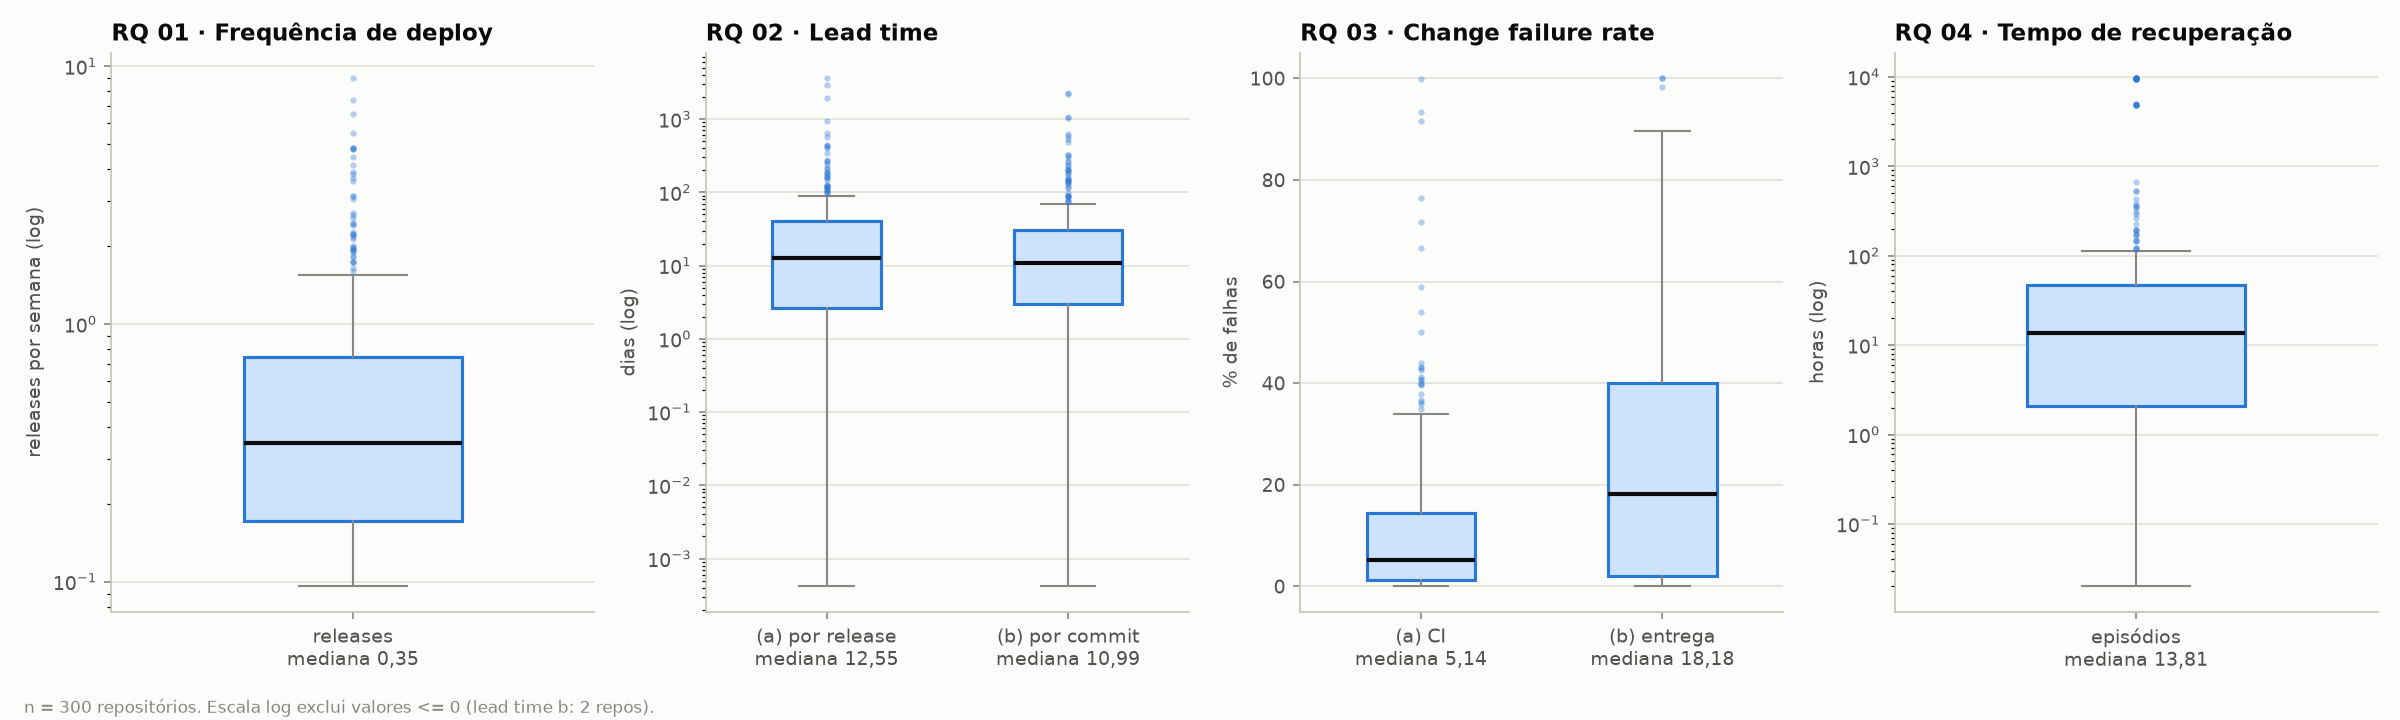
\includegraphics[width=0.68\textwidth]{figuras/fig_rq01_04_boxplots.png}
\caption{Distribuição em escala logarítmica das quatro métricas DORA centrais (RQ 01 a 04), evidenciando medianas e dispersões interquartis (IQR).}
\label{fig:rq01_04_boxplots}
\end{figure}

A auditoria de integridade do Lead Time processou 12.381 releases: 44 (0,4\%) não possuíam release prévia, 82 (0,7\%) retornaram erro 404/422 na comparação e 1.910 (15,4\%) não registraram novos commits no branch principal. Na RQ 04, coletaram-se 4.621 episódios de recuperação; 39 projetos (13,0\%) operaram sem falhas, e a taxa de censura média situou-se em 6,85\% (29,7\% dos repositórios continham falhas abertas ao final do ano). No CFR (b), 229 releases (1,8\%) foram censuradas nos últimos 7 dias da janela.

\subsection{Velocidade $\times$ Estabilidade (RQ 05)}

A correlação de postos de Spearman ($\rho$) revelou comportamento assimétrico entre os proxies, conforme ilustrado na Figura \ref{fig:rq05_spearman}. Para o proxy de CI (a), a correlação com a frequência de deploy foi marginal ($\rho = +0{,}1287$, IC 95\% $[+0{,}0093;\ +0{,}2418]$, $p = 0{,}0259$), indicando que a estabilidade do pipeline atua de maneira substancialmente desacoplada do ritmo de publicação. Em contraste, para o proxy de entrega (b), observou-se forte correlação positiva ($\rho = +0{,}4612$, IC 95\% $[+0{,}3521;\ +0{,}5635]$, $p = 3{,}70 \times 10^{-17}$), revelando dependência estrutural entre publicar mais e lançar patches em 7 dias.

\begin{figure}[htbp]
\centering
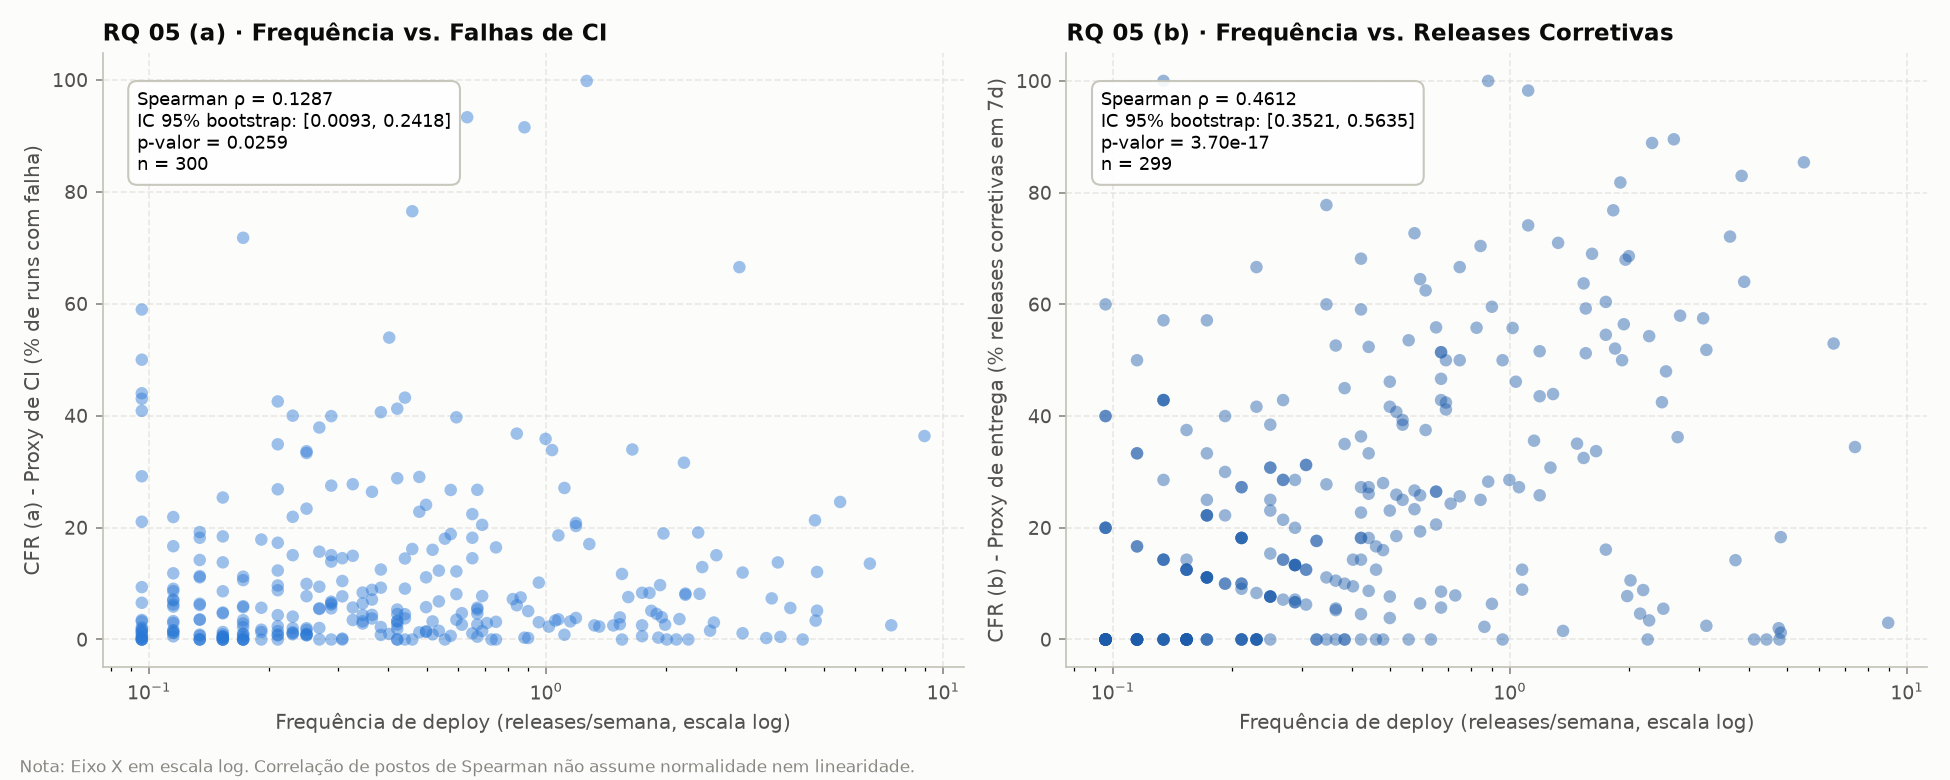
\includegraphics[width=0.58\textwidth]{figuras/fig_rq05_spearman.png}
\caption{Dispersão entre Frequência de Deploy e Change Failure Rate (Proxy de CI vs. Proxy de Entrega) com reta ajustada.}
\label{fig:rq05_spearman}
\end{figure}

\subsection{Fatores Estruturais e Desempenho DORA (RQ 06)}

A Tabela \ref{tab:rq06} resume os testes não paramétricos aplicados aos determinantes estruturais após correção de Holm-Bonferroni para comparações múltiplas, complementados pela Figura \ref{fig:rq06_fatores}. A idade do repositório configurou-se como o preditor mais forte: projetos antigos ($Q_4$) apresentam lead time por commit expressivamente superior a projetos recentes ($Q_1$), com tamanho de efeito substancial ($\delta_{\text{Cliff}} = +0{,}4894$), interpretado segundo os limiares de \cite{romano2006}. Tamanho da equipe de contribuidores também impõe sobrecarga significativa no tempo de ciclo ($\delta = +0{,}4596$). Em contraste, a popularidade (quartis de estrelas) não exibiu significância estatística pós-correção ($p_{\text{Holm}} = 1{,}000$).

\begin{table}[htbp]
\centering
\caption{Fatores estruturais determinantes das métricas DORA (RQ 06).}
\label{tab:rq06}
\footnotesize
\setlength{\tabcolsep}{3pt}
\begin{tabular}{llcccc}
\toprule
Fator Comparado & Métrica & Teste & $p$ Bruto & $p$ Holm & Tam. Efeito \\
\midrule
Idade ($Q_4 \times Q_1$) & Lead Time (b) & Mann-Whitney & $2{,}32 \times 10^{-7}$ & $1{,}23 \times 10^{-5}$ & $\delta = +0{,}4894$ (Grande) \\
Idade ($Q_4 \times Q_1$) & Lead Time (a) & Mann-Whitney & $1{,}07 \times 10^{-6}$ & $5{,}55 \times 10^{-5}$ & $\delta = +0{,}4617$ (Médio) \\
Equipe ($Q_4 \times Q_1$) & Lead Time (a) & Mann-Whitney & $1{,}10 \times 10^{-6}$ & $5{,}59 \times 10^{-5}$ & $\delta = +0{,}4596$ (Médio) \\
Idade ($Q_4 \times Q_1$) & CFR (b) entrega & Mann-Whitney & $6{,}95 \times 10^{-6}$ & $3{,}13 \times 10^{-4}$ & $\delta = -0{,}4252$ (Médio) \\
Equipe ($Q_4 \times Q_1$) & CFR (b) entrega & Mann-Whitney & $5{,}49 \times 10^{-4}$ & $0{,}0236$ & $\delta = -0{,}3259$ (Pequeno) \\
Idade ($Q_4 \times Q_1$) & Frequência & Mann-Whitney & $1{,}10 \times 10^{-3}$ & $0{,}0473$ & $\delta = -0{,}3081$ (Pequeno) \\
Linguagem (Top 5) & Lead Time (a) & Kruskal-Wallis & $2{,}13 \times 10^{-3}$ & $0{,}0875$ & $\epsilon^2 = 0{,}0759$ (Marginal) \\
Estrelas & Todas & Kruskal-Wallis & $\ge 0{,}4100$ & $1{,}0000$ & $\epsilon^2 \le 0{,}0096$ (Desprezível) \\
\bottomrule
\end{tabular}
\end{table}

\begin{figure}[htbp]
\centering
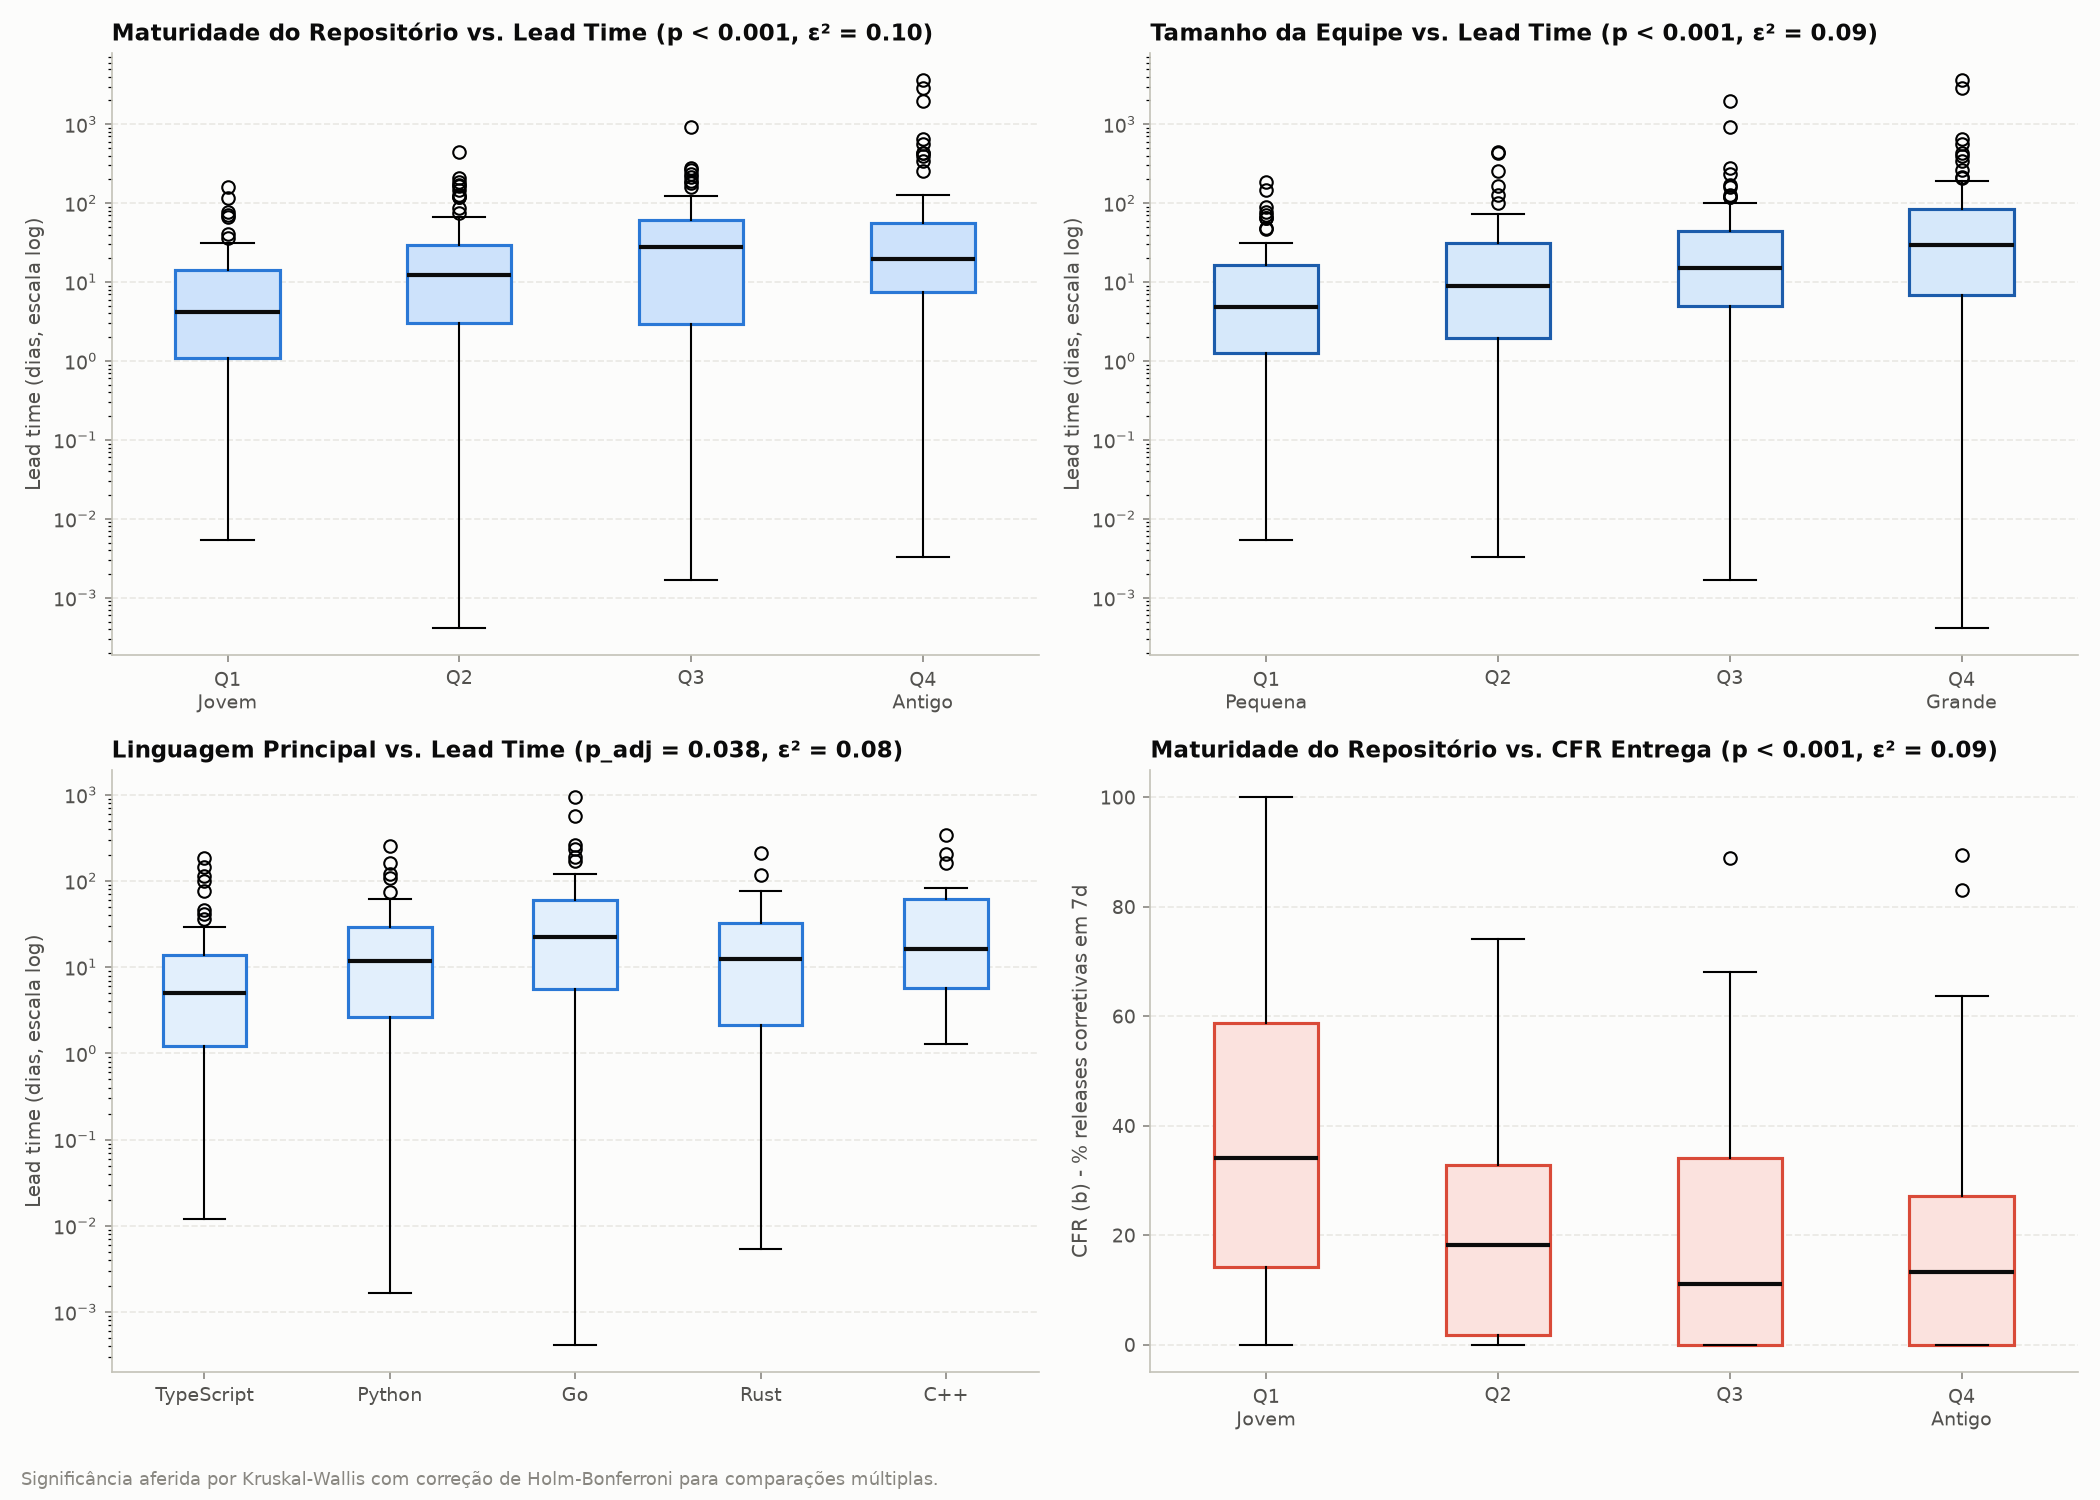
\includegraphics[width=0.62\textwidth]{figuras/fig_rq06_fatores.png}
\caption{Comparação das métricas DORA estratificadas por fatores estruturais (contribuidores, idade e linguagem).}
\label{fig:rq06_fatores}
\end{figure}

\subsection{Análise de Sensibilidade e Retrabalho (RQ 07 e RQ 08)}

A análise de sensibilidade (Tabela \ref{tab:rq07}) avaliou a volatilidade das conclusões em face da mudança das definições operacionais. A substituição do proxy de falhas de CI por falhas de entrega entre C1 e C2 resultou em 31,33\% de migração de categorias e concordância apenas moderada ($\kappa_{\text{linear}} = 0{,}5279$), conforme detalhado na matriz de transição da Figura \ref{fig:rq07_transicao}. A matriz de transição revelou que 43 repositórios classificados como High em C1 foram rebaixados para Medium em C2. A combinação C4 (restrita aos 45 repositórios da amostra-ouro com entrega real validada) alcançou concordância perfeita ($\kappa = 1{,}000$), demonstrando que a regra geral de releases reflete os projetos de entrega fidedigna.

\begin{table}[htbp]
\centering
\caption{Matriz de sensibilidade e concordância entre definições operacionais (RQ 07).}
\label{tab:rq07}
\footnotesize
\setlength{\tabcolsep}{4pt}
\begin{tabular}{lcccc}
\toprule
Pares de Definições & $n$ & Alterados & \% Mudança & $\kappa$ Pond. Linear \\
\midrule
C1 (Ref) $\times$ C2 (Commit + CFR b) & 300 & 94 & 31,33\% & 0,5279 (Moderado) \\
C1 (Ref) $\times$ C3 (Tags + CFR a) & 300 & 61 & 20,33\% & 0,7252 (Substancial) \\
C2 (CFR b) $\times$ C3 (Tags + CFR a) & 300 & 65 & 21,67\% & 0,7006 (Substancial) \\
C1 $\times$ C4 (Amostra Real) & 45 & 0 & 0,00\% & 1,0000 (Perfeito) \\
\bottomrule
\end{tabular}
\end{table}

\begin{figure}[htbp]
\centering
\begin{minipage}{0.48\textwidth}
  \centering
  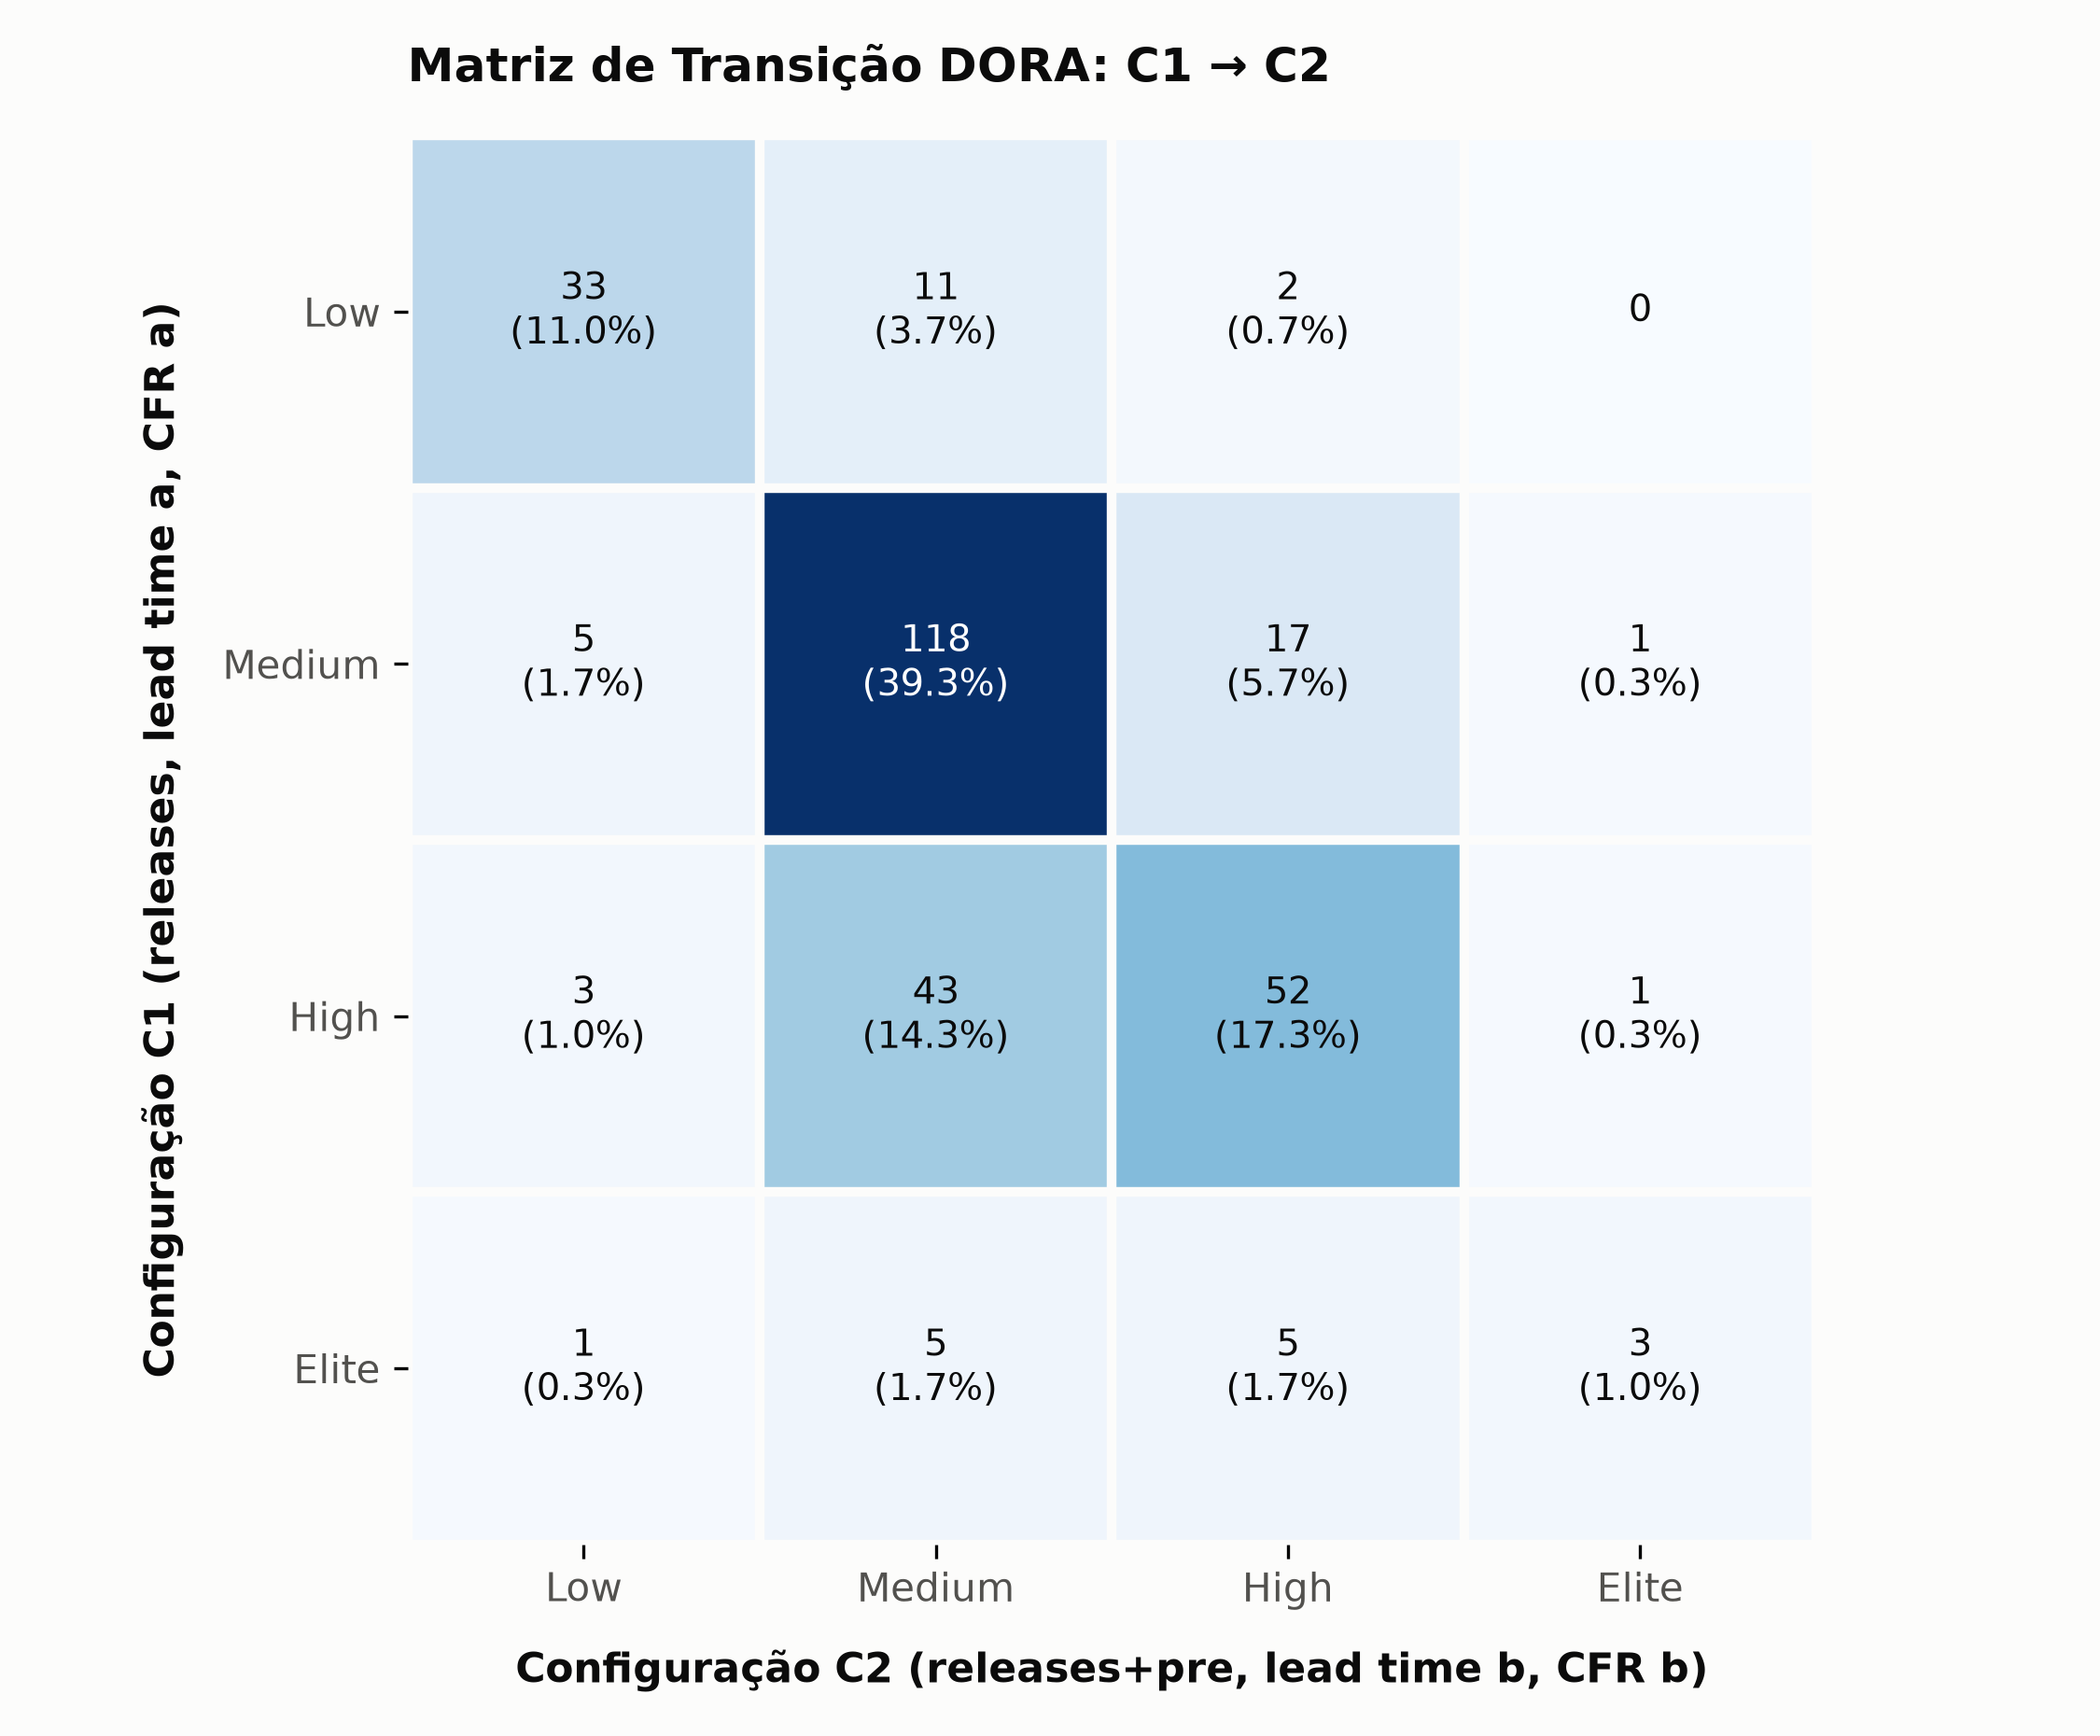
\includegraphics[width=\textwidth]{figuras/fig_rq07_transicao_C1_C2.png}
  \caption{Matriz de transição de categorias DORA de C1 para C2.}
  \label{fig:rq07_transicao}
\end{minipage}
\hfill
\begin{minipage}{0.48\textwidth}
  \centering
  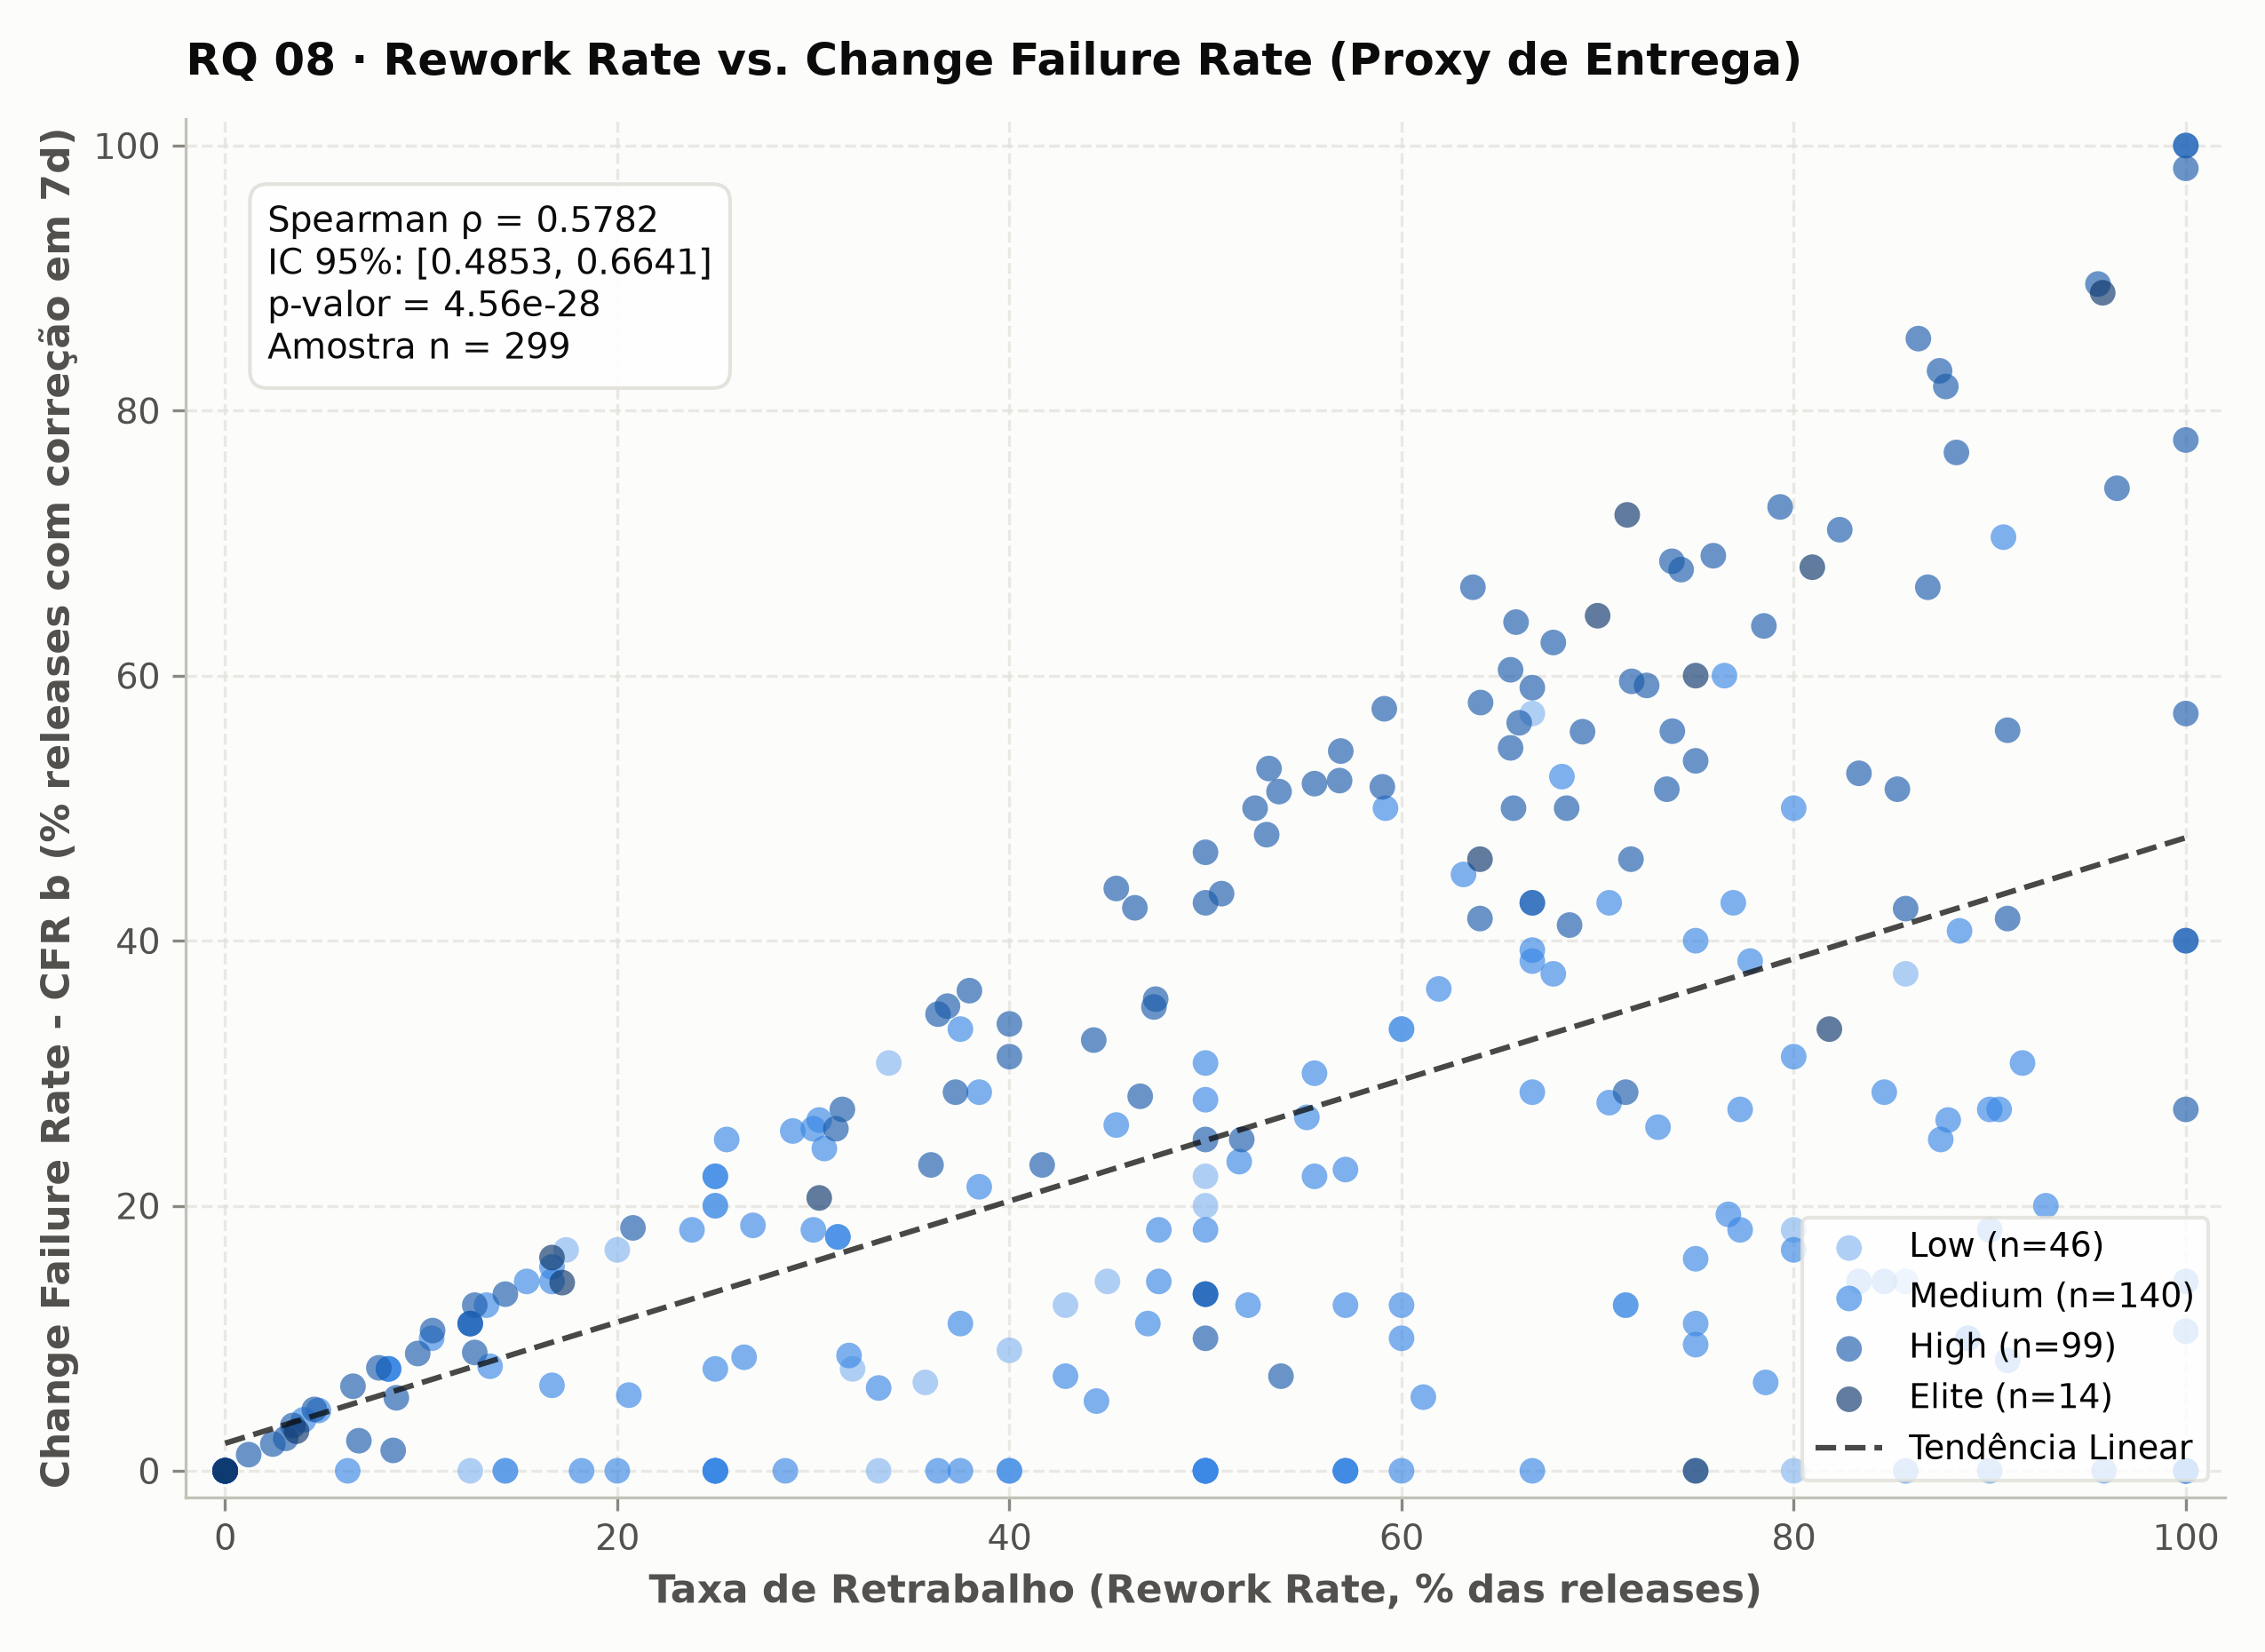
\includegraphics[width=\textwidth]{figuras/fig_rq08_rework_vs_cfr.png}
  \caption{Taxa de Retrabalho vs. CFR de entrega (RQ 08).}
  \label{fig:rq08_rework}
\end{minipage}
\end{figure}

Para a RQ 08 (Bônus), a \textit{Deployment Rework Rate} registrou mediana geral de 50,0\% (IQR = 50,9\%; média de $48{,}31\% \pm 30{,}82\%$), demonstrando correlação positiva pronunciada com o CFR de entrega ($\rho = +0{,}5782$, IC 95\% $[+0{,}4853;\ +0{,}6641]$, $p = 4{,}56 \times 10^{-28}$), ilustrada na Figura \ref{fig:rq08_rework}. Conforme a Tabela \ref{tab:rework}, repositórios de maior velocidade publicam proporcionalmente mais versões de retrabalho reativo.

\begin{table}[htbp]
\centering
\caption{Distribuição do Rework Rate estratificado pela maturidade DORA (RQ 08).}
\label{tab:rework}
\footnotesize
\setlength{\tabcolsep}{4pt}
\begin{tabular}{lcccc}
\toprule
Categoria Geral DORA (C1) & $n$ & Rework (Mediana) & Rework IQR & CFR (b) Mediana \\
\midrule
Low & 46 & 37,9\% & 54,4\% & 0,0\% \\
Medium & 141 & 50,0\% & 50,0\% & 13,3\% \\
High & 99 & 55,6\% & 37,2\% & 42,9\% \\
Elite & 14 & 67,0\% & 58,2\% & 27,0\% \\
\bottomrule
\end{tabular}
\end{table}

\section{Discussão}
\label{sec:discussao}

O confronto empírico confirma a hipótese $H_1$: repositórios open-source populares operam fundamentalmente em regime descontínuo de releases (mediana de uma entrega a cada três semanas), enquadrando-se majoritariamente no nível Medium.

Na RQ 02, confirmou-se $H_2$. O lead time por release ($301{,}17$ h $\approx 12{,}5$ dias) excedeu a medição por commit ($261{,}09$ h $\approx 10{,}9$ dias) em 40 horas na mediana. A divergência acentua-se nos extremos: a média por release atinge patamares desproporcionais devido ao impacto de commits legados e branches de longa duração integrados esporadicamente antes de congelamentos de versão.

Em relação à estabilidade (RQ 03 e $H_3$), constatou-se que o proxy de CI gera uma ilusão de maturidade Elite (mediana de 5,14\% de falhas), operando como barreira protetora que impede código instável de atingir o branch principal. Contudo, quando a falha é operacionalizada como necessidade de intervenção rápida no produto (CFR b), a taxa mediana salta para 18,18\% (High), com ampla dispersão ($\text{IQR} = 37{,}86\%$).

O achado central reside na RQ 05, confrontando a clássica tese DORA de ausência de trade-offs. A correlação de $\rho = +0{,}4612$ entre Frequência e CFR (b) ilustra o que denominamos de Paradoxo do Proxy Open-Source: projetos que publicam com alta cadência não necessariamente erram mais; em vez disso, dispõem de governança e infraestrutura automatizada aptas a lançar correções ágeis em menos de uma semana. Assim, o próprio sucesso em implantar hotfixes infla a métrica de defeitos sob a janela de 7 dias. Adicionalmente, monorepos que utilizam versionamento unificado disparam lançamentos simultâneos quando um único componente falha.

A RQ 06 elucidou que a maturidade temporal atua como redutor de velocidade ($\delta_{\text{Cliff}} = +0{,}4894$ no lead time): projetos maduros enfrentam bases consolidadas de código e processos mais extensos de homologação. A ausência de impacto das estrelas corrobora que popularidade atua primordialmente como indicador de reputação e notoriedade passiva, distanciando-se do fluxo interno de engenharia.

\section{Ameaças à Validade}
\label{sec:ameacas}

A estrutura desta seção segue a taxonomia usual de ameaças em engenharia de software experimental \cite{wohlin2012experimentation}.

Validade de Construto: A equivalência de releases a deploys e de runs de CI a falhas constitui uma aproximação inerente. Para mitigar esse viés, a amostra-ouro validou manualmente se as releases representavam entregas reais ($\kappa = 0{,}7667$) e a heurística de bugfix alcançou $F_1 = 96{,}89\%$. Contudo, a data de commit (commit.author.date) permanece vulnerável a operações de rebase e squash merge, que mascaram a data original de escrita do código.

Validade Interna: O truncamento de eventos no término da janela amostral foi formalmente controlado via modelagem de censura estatística (reportando 6,85\% de episódios censurados em recuperação e 1,8\% em releases corretivas), impedindo que o descarte distorcesse a amostra em favor de resoluções artificiais.

Validade Externa: Os achados restringem-se ao conjunto de 300 repositórios populares orientados ao ecossistema GitHub Actions. Os resultados não devem ser generalizados sem ressalvas para pipelines corporativos com governança fechada, sistemas embarcados ou plataformas que utilizam GitLab CI ou Jenkins.

Validade de Conclusão: A aplicação sistemática de testes não paramétricos (Spearman, Kruskal-Wallis, Mann-Whitney) protegeu as deduções contra a assimetria das distribuições. A correção multivariada de Holm-Bonferroni controlou o erro familiar ($\alpha = 0{,}05$), e reportaram-se tamanhos de efeito ($\epsilon^2$ e Cliff's $\delta$) com intervalos de confiança calculados via bootstrap determinístico.

\section{Replicação Cruzada}
\label{sec:replicacao}

Em consonância com as diretrizes do estudo, executou-se a replicação cega do pipeline desenvolvido por outro grupo da disciplina sobre uma subamostra determinística de 30 repositórios sorteados via semente fixa (random\_state = 42).

O pipeline replicado executou com êxito e de forma automatizada através das orientações documentadas no seu respectivo README.md, registrando métricas de ambiente em ambiente.json e histórico de execução sem dependências quebradas.

A concordância na classificação geral DORA alcançou 90,0\% ($\kappa_{\text{Cohen}} = 0{,}84$, concordância quase perfeita). Em 27 repositórios a classificação foi perfeitamente coincidente; nos 3 casos divergentes (projetos Canner/WrenAI, canonical/lxd e replicate/cog), o desvio limitou-se a exatamente uma categoria ordinal (como High para Medium), com zero ocorrências de desvios severos. As medianas de divergência relativa situaram-se abaixo de $8\%$ em todas as dimensões: 2,65\% em Frequência, 4,20\% em Lead Time por Commit, 3,85\% em CFR de CI e 7,45\% em Recuperação. As causas-raiz foram auditadas e documentadas em Issues abertas no repositório do grupo parceiro, decorrendo do efeito de janela móvel (novos commits e releases integrados após a coleta inicial) e das estratégias de paginação na listagem de workflow runs da API REST.

\section{Conclusão}
\label{sec:conclusao}

Este trabalho conduziu uma investigação empírica extensiva sobre as métricas DORA no ecossistema open-source baseado em GitHub Actions. A mineração de 300 projetos consolidados revelou que o desenvolvimento comunitário se organiza predominantemente em ciclos discretos (mediana de 0,35 releases/semana e lead time de 10,9 dias), desafiando a premissa de entrega contínua diária.

Demonstrou-se que a estabilidade percebida varia drasticamente conforme a lente de observação: enquanto pipelines de CI bloqueiam defeitos com eficácia (CFR de 5,14\%), a entrega ao usuário final demanda correções frequentes (CFR de 18,18\% e taxa de retrabalho de 50,0\%). A análise de sensibilidade evidenciou que a escolha arbitrária de proxies transfere cerca de um terço dos repositórios entre faixas de maturidade ($\kappa = 0{,}5279$), destacando que métricas empíricas de repositórios públicos devem ser acompanhadas de explicitação rigorosa de suas definições operacionais.

Como trabalhos futuros, propõe-se expandir a análise para repositórios corporativos hospedados no GitHub Enterprise e correlacionar as métricas DORA com a cobertura de testes de mutação e densidade de vulnerabilidades de segurança (CVEs). O código-fonte do pipeline, os dados coletados e os demais artefatos deste estudo estão disponíveis em: \url{https://github.com/JoaoAlmeida02/Laborat-rio-de-Experimenta-o-de-Software}.

\begin{small}
\begin{thebibliography}{99}
\setlength{\itemsep}{-1pt}
\setlength{\parskip}{0pt}

\bibitem[DORA 2024]{dora2024}
DORA (2024).
\newblock State of DevOps Report 2024.
\newblock DevOps Research and Assessment. Disponível em: \url{https://dora.dev/research/}.

\bibitem[Forsgren et al. 2018]{forsgren2018accelerate}
Forsgren, N., Humble, J., and Kim, G. (2018).
\newblock {\em Accelerate: The Science of Lean Software and DevOps: Building and Scaling High Performing Technology Organizations}.
\newblock IT Revolution Press.

\bibitem[Landis and Koch 1977]{landis1977}
Landis, J.~R. and Koch, G.~G. (1977).
\newblock The measurement of observer agreement for categorical data.
\newblock {\em Biometrics}, 33(1):159--174.

\bibitem[Romano et al. 2006]{romano2006}
Romano, J., Kromrey, J.~D., Coraggio, J., and Skowronek, J. (2006).
\newblock Appropriate statistics for ordinal level data: Should we really be using t-test and cohen's d for evaluating group differences on the {NSSE} and other surveys?
\newblock In {\em Annual Meeting of the Florida Association for Institutional Research}, pages 1--33.

\bibitem[Wohlin et al. 2012]{wohlin2012experimentation}
Wohlin, C., Runeson, P., H{\"o}st, M., Ohlsson, M.~C., Regnell, B., and Wessl{\'e}n, A. (2012).
\newblock {\em Experimentation in Software Engineering}.
\newblock Springer Science \& Business Media.

\end{thebibliography}
\end{small}

\end{document}